% This template was originally by R. Jacob Vogelstein
% Updated on March 1, 2010 by Noah J. Cowan

\documentclass[12pt,letterpaper, oneside,final]{template/thesisClass}
\special{papersize=8.5in,11in}
\pdfpagewidth 8.5in
\pdfpageheight 11.0in
\makeatletter
\let\@currsize\normalsize
\makeatother
\usepackage{acronym}
\usepackage{cite}
\usepackage{amsmath,amsfonts}
\usepackage{graphicx}
\graphicspath{{./figs/}}
\usepackage{fixltx2e}
\usepackage{array}
% wrapfig is fragile: use sparingly
\usepackage{wrapfig}
%\usepackage{times}  % Use this for ugly fonts
\usepackage[dvipsnames]{xcolor}
\usepackage{fancyhdr}    % Use nice looking headers along with the required footer page numbers
\usepackage{ifthen}
\usepackage{lettrine}
\usepackage{multirow}
\usepackage{hyperref}
%\usepackage[document]{ragged2e}
\usepackage{caption}
\usepackage{epigraph}
\usepackage{setspace}

%\usepackage[hypertex]{hyperref}

%Define the header/footer style
\pagestyle{fancy}
\fancyhf{}

\setlength{\headheight}{15pt}
%\lhead{\leftmark}
\cfoot{\thepage}
\renewcommand{\headrulewidth}{0pt}
\fancypagestyle{plain}{% Redefine ``plain'' style for chapter boundaries
\fancyhf{} % clear all header and footer fields

\fancyfoot[C]{\thepage} % except the center
\renewcommand{\headrulewidth}{0pt}
\renewcommand{\footrulewidth}{0pt}}
%\renewcommand\chaptername{}
%\renewcommand\chaptermark{1}
\renewcommand{\chaptermark}[1]{\markboth{ }{}}
\newcommand{\HRule}{\rule{\linewidth}{0.5mm}} % New command to make the lines in the title page
\newcommand{\notes}[1]{\textcolor{black}{\textbf{#1}}}


%\tolerance=10000

%\makeglossary % enable the glossary

\begin{document}

\title{AIM LAB SAMPLE DISSERTATION TEMPLATE}
\author{Weijian Shang}
\degreemonth{June}
\degreeyear{2014}
\dissertation
\doctorphilosophy
\copyrightnotice

% add your chapters, best way is to have separate TeX files for each chapter
%% FRONTMATTER

\begin{frontmatter}

% generate title
\maketitle

\pagebreak
\vskip 2em
         {Approved by:\par}
         \vskip 1em
         \vspace{10 mm}
         \ssp\rule[-2pt]{8cm}{0.5pt}\par
         {Prof. Gregory S. Fischer, Advisor\par}
         {Worcester Polytechnic Institute\par}

         \vskip 1em
         \vspace{10 mm}
         \ssp\rule[-2pt]{8cm}{0.5pt}\par
         {Prof. First M. Last, Committee Member\par}
         {Worcester Polytechnic Institute\par}

         \vskip 1em
         \vspace{10 mm}
         \ssp\rule[-2pt]{8cm}{0.5pt}\par
         {Prof. First M. Last, Committee Member\par}
         {Worcester Polytechnic Institute\par}

         \vskip 1em
         \vspace{10 mm}
         \ssp\rule[-2pt]{8cm}{0.5pt}\par
         {Prof. First M. Last, Committee Member\par}
         {Johns Hopkins University\par}

         \vskip 1em
         \vspace{10 mm}
         \ssp\rule[-2pt]{8cm}{0.5pt}\par
         {Prof. First M. Last, Committee Member\par}
         {Brigham and Women's Hospital, Harvard Medical School \par}

         \vskip 1em
         \vspace{10 mm}
         \ssp\rule[-2pt]{8cm}{0.5pt}\par
         {Prof. First M. Last, Graduate Committee Representative\par}
         {Worcester Polytechnic Institute\par}

\begin{abstract}

This is abstract.

\end{abstract}

\begin{acknowledgment}

I would like to express my gratitude to everybody in the world.

\end{acknowledgment}

\begin{dedication}

This dissertation is dedicated to everybody in the world.

\end{dedication}

% generate table of contents
\tableofcontents

% generate list of tables
\listoftables

% generate list of figures
\listoffigures

Disclaimer: certain materials are included under the fair use exemption of the U.S. Copyright Law and have been prepared according to the fair use guidelines and are restricted from further use.

\pagebreak
\section*{Acronyms}
\begin{acronym}
\acro{MRI}{Magnetic Resonance Imaging}
\acro{NIH}{National Institutes of Health}
\acro{SNR}{Signal-to-Noise Ratio}

\end{acronym}

\end{frontmatter}

\chapter{Introduction}
\label{intro} % Always give a unique label

\epigraph{``All children are artists. The problem is how to remain an artist once he grows up."(This is not necessary if you don't want it.)}
{Pablo Picasso}

This is the introduction.

\section{Background}
\label{sec:S1}

This is the background of introduction.

Some text.

\subsection{Sub Section 1}
\label{sec:SS1}

This is the sub section 1 of background.

\subsection{Sub Section 2}
\label{sec:SS2}

This is the sub section 2 of background.



\section{Literature Review}
\label{sec:InterventionRobotics}

This is the Literature Review Section. Here is a figure: Fig.\ref{fig:exampleFigure} and here is a table: Table \ref{tab:Protocol}.

\begin{figure}[h]
  \begin{center}
    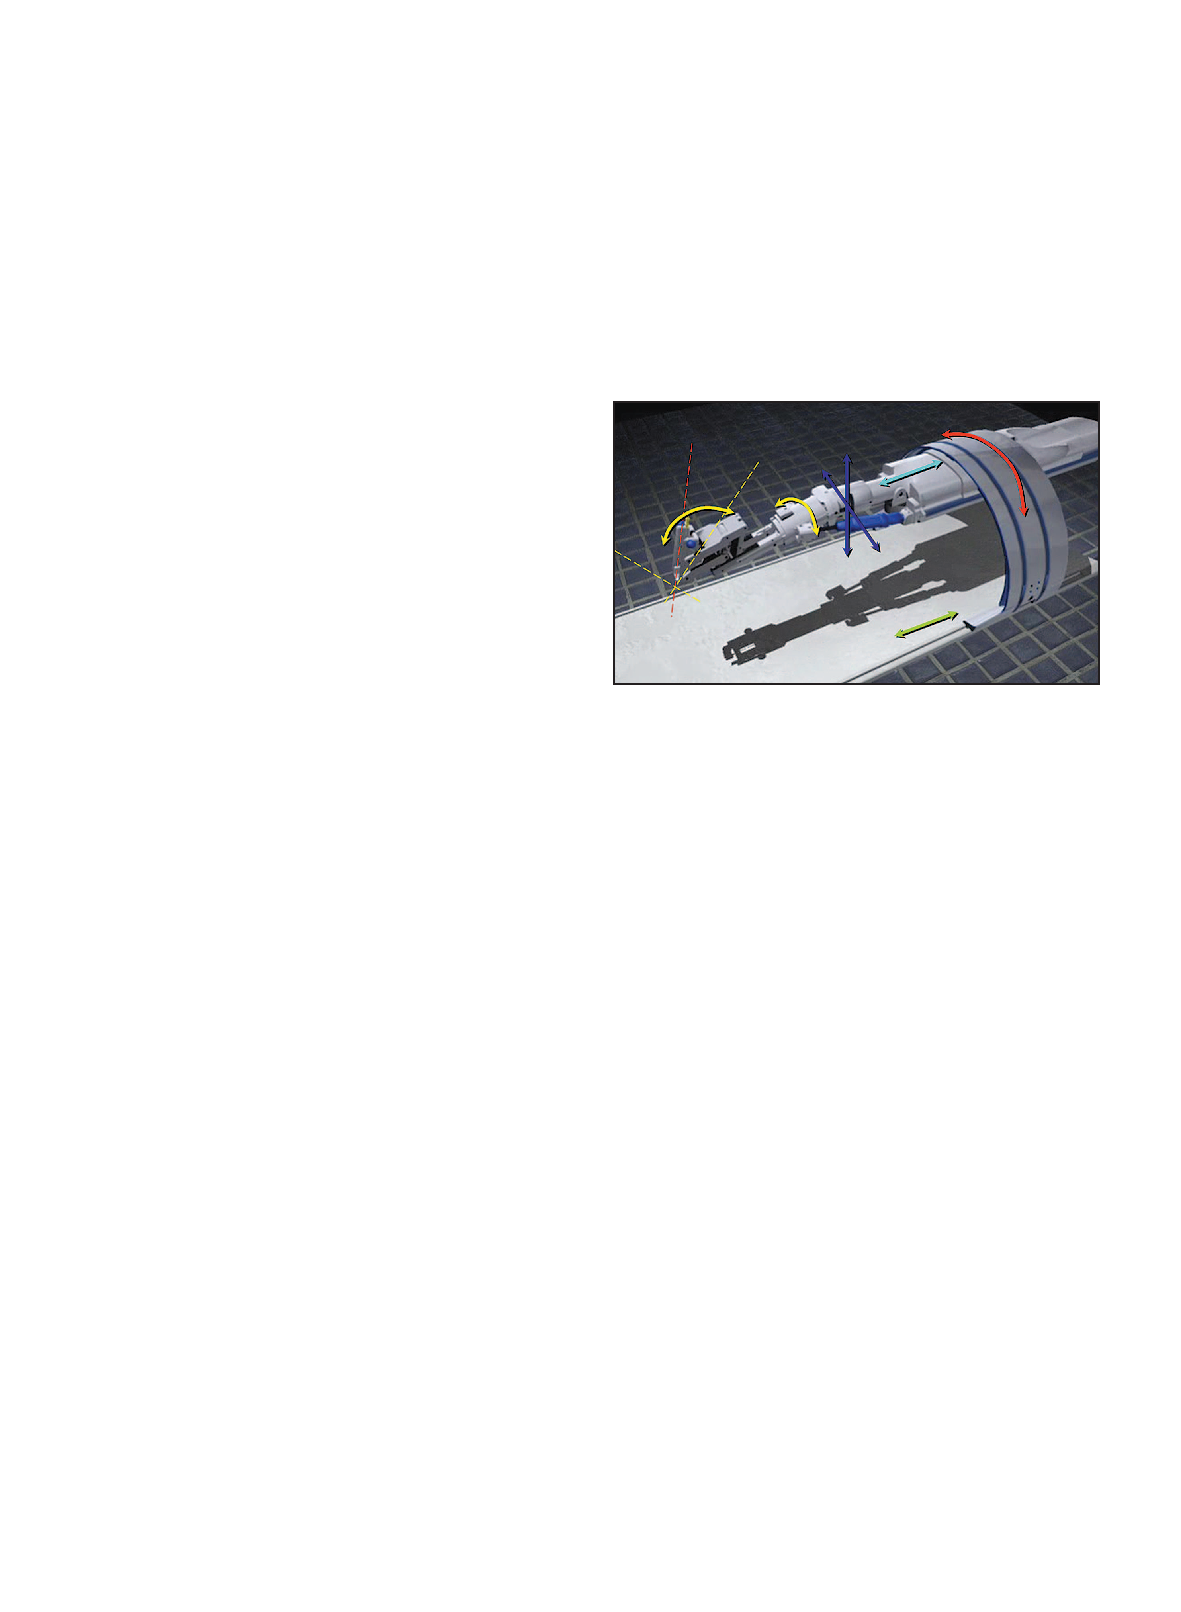
\includegraphics[width=120mm]{fig/chap1/innomotion.pdf}
  \end{center}
  \vspace{-4mm}
\caption[CAD model of the Innomotion robotic system.]
{This is a sample figure with a sample citation \cite{Fischer2008_TMECH} \copyright 2008 IEEE.}
 \label{fig:exampleFigure}
\vspace{-2mm}
\end{figure}

\begin{table}[htb]
  \begin{center}
\caption[Scan parameters for compatibility evaluation.]{Detailed scan parameters for each of four protocols for compatibility evaluation}
\label{tab:Protocol}
  \end{center}
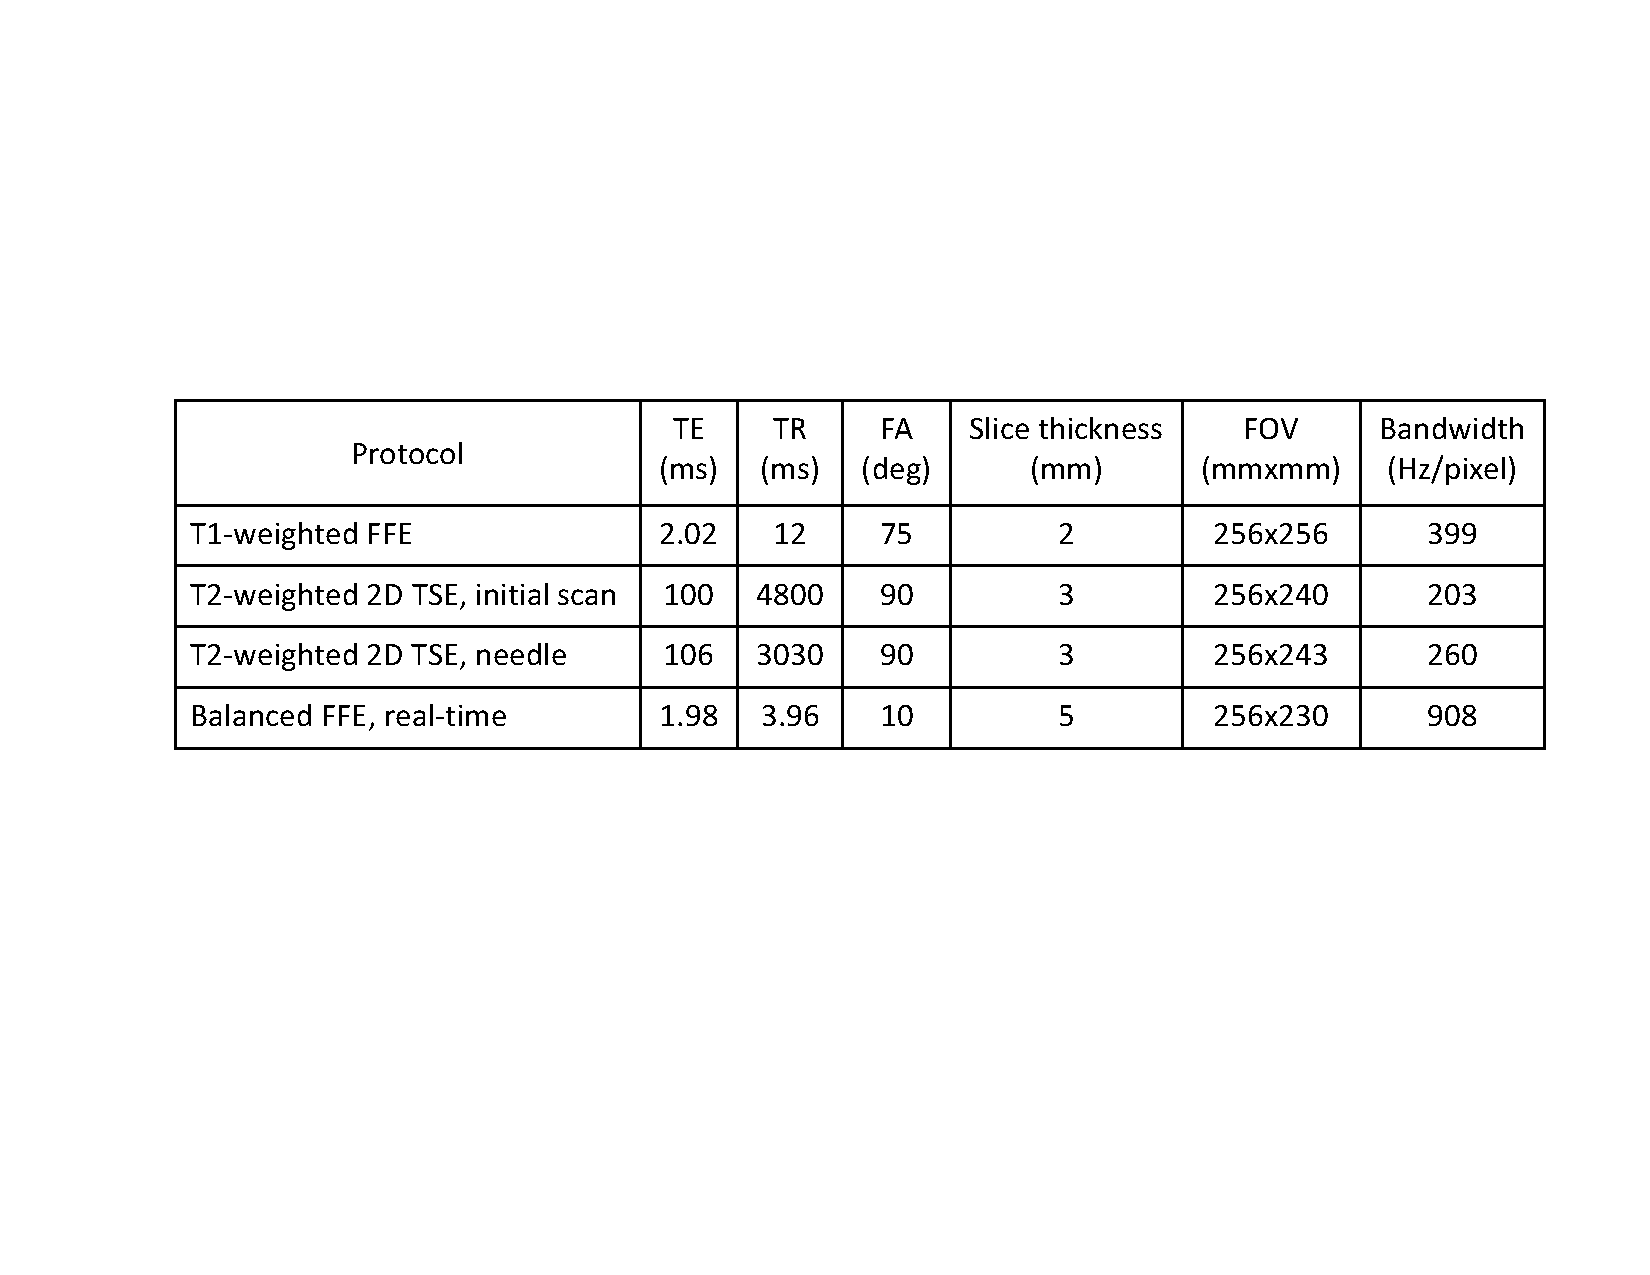
\includegraphics[width=150mm]{fig/chap1/protocol.pdf}
%\caption*{}
\end{table}
\vspace{-2mm}

\section{Dissertation Contributions}
\label{sec:Contributions}

\begin{itemize}
\item
\textbf{Contribution 1}

Contribution 1

\item
\textbf{Contribution 2}

Contribution 2

\item
\textbf{Contribution 3}

Contribution 3

\end{itemize}


\section{Dissertation Overview}
\label{sec:Overview}

This introductory chapter presents ...

Chapter 2 introduces ...

Chapter 3 describes ...

Chapter 4 presents ...

Chapter 5 summarizes ...

Chapter 6 presents ...

We conclude and discuss future work in Chapter 7. 
%%%%%%%%%%%%%%%%%%%%% chapter.tex %%%%%%%%%%%%%%%%%%%%%%%%%%%%%%%%%
%
% sample chapter
%
% Use this file as a template for your own input.
%
%%%%%%%%%%%%%%%%%%%%%%%% Springer-Verlag %%%%%%%%%%%%%%%%%%%%%%%%%%

%\begin{savequote}[8cm]
%  ``Veni, vidi, vici.''
%  \qauthor{Julius Caesar}
%\end{savequote}


\chapter{My Work}
\label{intro} % Always give a unique label
% use \chaptermark{}
% to alter or adjust the chapter heading in the running head

\epigraph{``Veni, vidi, vici."}
{Julius Caesar}

This chapter introduces ...

\section{Introduction}
\label{sec:intro}

This is the introduction.

\subsection{Sub Section 1}
\label{sec:S2SS1}

This is the sub section 1 of intro.

\subsection{Sub Section 2}
\label{sec:S2SS2}

This is the sub section 2 of intro.

\section{My Work Part 1}
\label{sec:p1}

This is part 1 of my work.

\section{My Work Part 2}
\label{sec:p2}

This is part 2 of my work.

\section{My Work Part 3}
\label{sec:p3}

This is part 3 of my work.

\section{Discussion and Conclusions}
\label{section:Discussionconclusion}

This is the discussion and conclusions for this section.
\chapter{Conclusions and Future Extension}
\label{intro} % Always give a unique label

\epigraph{``Prediction is very difficult, especially about the future."}
{Niels Bohr}

This dissertation discussed ...


\section{Summary of Work and Contributions}
An overview of this work is presented below with a summary of contributions and lessons learned along the way.

\begin{itemize}
\item
\textbf{Contribution 1}

Contribution 1

\item
\textbf{Contribution 2}

Contribution 2

\item
\textbf{Contribution 3}

Contribution 3

\end{itemize}

\section{Impact and Future Work}
The research presented in this dissertation addresses several major challenges.

%\begin{itemize}
\textbf{Impact}

Here is the impact of my work.

%\item 
\textbf{Lessons Learned}

Some lessons I've learned.

%\item 
\textbf{Future Work}

Future work includes...

%\end{itemize}

%% REFERENCES
% if you use BIBTEX
\begin{spacing}{1}
\def\dsp{\def\baselinestretch{1.25}\large\normalsize}
\bibliographystyle{template/IEEEtran}
\bibliography{bibliography}
\end{spacing}
\end{document}
